\documentclass[11pt,a4paper]{article}

\usepackage[margin=2.5cm]{geometry}
\usepackage[T1]{fontenc}
\usepackage{lmodern}
\usepackage{microtype}
\usepackage{booktabs}
\usepackage{longtable}
\usepackage{xcolor}
\usepackage{listings}
\usepackage{amsmath}
\usepackage{amssymb}
\usepackage{enumitem}
\usepackage{tikz}
\usetikzlibrary{arrows.meta,positioning}
\usepackage[hidelinks]{hyperref}

\definecolor{codebg}{RGB}{247,247,247}
\definecolor{codekey}{RGB}{20,80,160}
\definecolor{codestr}{RGB}{150,60,20}

\lstdefinestyle{json}{
  basicstyle=\ttfamily\footnotesize,
  backgroundcolor=\color{codebg},
  breaklines=true, columns=fullflexible, keepspaces=true,
  showstringspaces=false, frame=single, framerule=0pt, framesep=6pt,
  xleftmargin=6pt, stringstyle=\color{codestr},
  literate=*{:}{{{\color{codekey}:}}}{1}{\{}{{{\color{codekey}\{}}}{1}{\}}{{{\color{codekey}\}}}}{1},
}
\lstdefinestyle{plain}{
  basicstyle=\ttfamily\footnotesize, backgroundcolor=\color{codebg},
  breaklines=true, columns=fullflexible, keepspaces=true,
  showstringspaces=false, frame=single, framerule=0pt, framesep=6pt, xleftmargin=6pt,
}
\lstset{style=json}

\newcommand{\code}[1]{\texttt{\small #1}}
\newcommand{\file}[1]{\texttt{\small #1}}

% ---- GitHub links to files in the repository ---------------------------------
\newcommand{\ghbase}{https://github.com/ArashMassoudieh/OpenHydroQual/blob/master}
\newcommand{\ghtree}{https://github.com/ArashMassoudieh/OpenHydroQual/tree/master}
\newcommand{\exfile}[1]{\href{\ghbase/#1}{\file{#1}}}
\newcommand{\exdir}[1]{\href{\ghtree/#1}{\file{#1}}}

\title{\textbf{The SCS Curve Number Catchment in OpenHydroQual}\\[0.3em]
       \large Formulation, unit hydrograph routing, and reference}
\author{}
\date{}

\begin{document}
\maketitle
\vspace{-2.5em}

\begin{abstract}
\noindent
The SCS (NRCS) Curve Number method is an event-based, cumulative procedure: it
maps total rainfall onto total runoff and says nothing about rates. This
document sets out how it is recast as a system of ordinary differential
equations so that it can live inside a continuous simulator, shows that the
recast form reproduces the original algebraic method exactly, describes the
routing that turns runoff volume into an outlet hydrograph, and documents the
resulting OpenHydroQual component and its parameters.
\end{abstract}

\tableofcontents

\section{The classical method}

For a storm of cumulative depth $P$, the curve number method gives cumulative
direct runoff

\begin{equation}
Q=\frac{(P-I_a)^{2}}{P-I_a+S},\qquad P>I_a,
\label{eq:scs}
\end{equation}

\noindent
and $Q=0$ otherwise, where $S$ is the maximum potential retention after runoff
begins and $I_a$ the initial abstraction. $S$ follows from the curve number,

\begin{equation}
S=\frac{25400}{CN}-254 \ \ [\mathrm{mm}] \qquad\Longleftrightarrow\qquad
S=\frac{25.4}{CN}-0.254 \ \ [\mathrm{m}],
\label{eq:S}
\end{equation}

\noindent
and the standard closure is $I_a=0.2\,S$. Writing $P_e=P-I_a$ for effective
rainfall, the water not becoming runoff is the continuing retention

\begin{equation}
F=P_e-Q=\frac{S\,P_e}{P_e+S}.
\label{eq:F}
\end{equation}

Equation~\eqref{eq:scs} is a relation between two accumulated depths. It has no
time in it, which is why the method on its own produces a runoff \emph{volume}
and requires a separate unit hydrograph to produce a \emph{hydrograph}.

\section{Differential formulation}

\subsection{A single state}

Let $W$ be the \emph{total} abstraction depth --- the initial abstraction plus
the continuing retention --- so that $W=I_a+F$ and $W\to I_a+S=1.2\,S$ as the
storm grows. Define the runoff fraction

\begin{equation}
\boxed{\;C(W)=\left[\,1-\left(\frac{S+I_a-W}{S}\right)^{2}\right]^{+}\;}
\label{eq:C}
\end{equation}

\noindent
where $[\,\cdot\,]^{+}=\max(\cdot,0)$. The catchment is then two coupled
reservoirs driven by the rainfall rate $i(t)$ over an area $A$:

\begin{equation}
\frac{dV_W}{dt}=i\,A\,\bigl(1-C(W)\bigr)-k\,V_W,
\qquad
\frac{dV_1}{dt}=i\,A\,C(W)-\frac{V_1}{K},
\qquad W=\frac{V_W}{A}.
\label{eq:ode}
\end{equation}

\noindent
$V_W$ is the abstraction store, $V_1$ the surface store, and $k$ a drying
coefficient discussed in section~\ref{sec:recovery}. Rainfall is partitioned at
every instant: a fraction $C$ becomes runoff, the rest is abstracted.

\subsection{Why this is the classical method, exactly}

Two properties of \eqref{eq:C} do the work.

\paragraph{The initial abstraction is automatic.}
While $W<I_a$ the quantity $(S+I_a-W)/S$ exceeds unity, the bracket in
\eqref{eq:C} is negative, and the clamp gives $C=0$. \emph{No runoff whatever is
produced until $W=I_a$}, which is precisely the meaning of the initial
abstraction. From \eqref{eq:ode} with $C=0$ we get $dW/dt=i$, so all rainfall is
abstracted until the threshold is reached, and $W=P$ over that period. The
threshold is therefore crossed exactly when $P=I_a$.

\paragraph{Beyond the threshold, the curve number equation is recovered.}
For $W>I_a$, ignoring drying and dividing \eqref{eq:ode} by $i$,

\begin{equation}
\frac{dW}{dP}=1-C=\left(\frac{S+I_a-W}{S}\right)^{2}.
\end{equation}

\noindent
Substituting $u=S+I_a-W$, so that $du/dP=-u^{2}/S^{2}$, and integrating from
the threshold ($W=I_a$, $u=S$ at $P=I_a$):

\begin{equation}
\frac{1}{u}-\frac{1}{S}=\frac{P-I_a}{S^{2}}
\quad\Longrightarrow\quad
u=\frac{S^{2}}{P_e+S}
\quad\Longrightarrow\quad
W=I_a+\frac{S\,P_e}{P_e+S},
\end{equation}

\noindent
which is $I_a+F$ with $F$ exactly as in \eqref{eq:F}. The cumulative runoff is
then

\begin{equation}
Q=P-W=(I_a+P_e)-I_a-\frac{S\,P_e}{P_e+S}=\frac{P_e^{2}}{P_e+S},
\end{equation}

\noindent
identical to \eqref{eq:scs}. The differential form is a reformulation, not an
approximation.

\paragraph{Numerical behaviour.}
$C$ is continuous, rising from zero with slope $2/S$ at $W=I_a$, so there is no
discontinuous switch for the solver. The formulation is also self-limiting:
$C\to1$ only as $W\to1.2S$, and the retention rate $1-C$ vanishes there, so $W$
approaches its bound asymptotically and never needs clipping.

\subsection{Recovery between storms}\label{sec:recovery}

The curve number method is an event method. Without recovery, $W$ only
increases, $C\to1$, and the catchment becomes permanently impervious after
enough cumulative rain. The $-k\,V_W$ term in \eqref{eq:ode} empties the
abstraction store between events with time constant $1/k$, which should lie
between a typical storm duration and a typical inter-event time. Water removed
this way leaves the model; if it is needed downstream, the abstraction store
should instead discharge to a soil or groundwater block.

\section{The outlet hydrograph}

\subsection{Volume versus shape}

Equation~\eqref{eq:ode} determines how much water becomes runoff, and does so
exactly. It says nothing about \emph{when} that water arrives at the outlet.
Standard practice convolves the excess-rainfall series with the NRCS
dimensionless unit hydrograph. A continuous simulator does not convolve --- it
routes --- and the routing is what fixes the shape.

\subsection{Nash cascade}

Runoff is routed through $n$ equal linear reservoirs in series,

\begin{equation}
\frac{dV_j}{dt}=\frac{V_{j-1}}{K}-\frac{V_j}{K}\quad (j=2\ldots n),
\qquad q_{out}=\frac{V_n}{K},
\end{equation}

\noindent
the first of which is the surface store of \eqref{eq:ode}. The impulse response
of this chain is the gamma density

\begin{equation}
h(t)=\frac{1}{K\,\Gamma(n)}\left(\frac{t}{K}\right)^{n-1}e^{-t/K},
\end{equation}

\noindent
which is the continuous-time counterpart of a gamma unit hydrograph. Its time
to peak is $(n-1)K$.

\subsection{Matching the NRCS unit hydrograph}

\paragraph{Timing.} Set

\begin{equation}
\boxed{\;K=\frac{L}{n-1}\;}
\end{equation}

\noindent
where $L$ is the NRCS lag. The peak of the response then falls exactly at the
lag, for any $n$.

It is worth being explicit about a trap here. The familiar expression
$T_p=D/2+0.6\,T_c$ is the time to peak of a unit hydrograph of \emph{finite}
duration $D$. A continuous model convolves the \emph{instantaneous} unit
hydrograph, for which $D\to0$ and the correct target is the lag alone,
$L=0.6\,T_c$. Including the $D/2$ term would shift every hydrograph late by
half a rainfall interval.

\paragraph{Shape.} With the timing fixed, $n$ controls only how sharp the peak
is. The dimensionless peak of the gamma response, $h_{max}T_p$, is
$(n-1)^{n}e^{-(n-1)}/\Gamma(n)$; the NRCS dimensionless unit hydrograph with
its peak rate factor of 484 corresponds to approximately $0.75$:

\begin{center}
\begin{tabular}{@{}lccccc@{}}
\toprule
$n$ & 3 & 4 & \textbf{5} & 6 & NRCS target\\
\midrule
$h_{max}T_p$ & 0.54 & 0.67 & \textbf{0.78} & 0.87 & $\approx0.75$\\
\bottomrule
\end{tabular}
\end{center}

\noindent
so $n\approx4.7$, and $n=5$ is the closest integer. A caution on the
literature: values near $n\approx3.7$ are also quoted for the
``SCS-equivalent'' gamma hydrograph. That figure matches the fraction of volume
under the rising limb rather than the peak ordinate. The component here matches
the peak; $n=3$ is provided as a lighter alternative with a flatter peak and a
longer recession.

\subsection{Lag from catchment properties}

The NRCS lag equation is used, since it already involves the curve number and
is therefore consistent with the rest of the component:

\begin{equation}
L_{hr}=\frac{\ell^{0.8}\,(S'+1)^{0.7}}{1900\,\sqrt{Y}},
\qquad \ell\ [\mathrm{ft}],\quad S'=\frac{1000}{CN}-10\ [\mathrm{in}],\quad Y\ [\%].
\end{equation}

\noindent
Converting to metres and days, and writing the slope $s$ as a dimensionless
rise over run ($Y=100\,s$):

\begin{equation}
\boxed{\;L_{day}=\frac{\ell_m^{0.8}\left(\dfrac{1000}{CN}-9\right)^{0.7}}{176300\,\sqrt{s}}\;}
\qquad T_c=\frac{L}{0.6}.
\end{equation}

\noindent
The equation is calibrated for catchments below roughly $800$~ha with $CN$
between about 50 and 95; outside that range the lag should be supplied by other
means. Note that only $L$ is needed, since $K=L/(n-1)$; the time of
concentration is a diagnostic.

\section{Implementation}

\subsection{Structure}

The component is a composite of $n+1$ blocks. Rainfall falls on the surface
reservoir $R_1$; the partition link removes the abstracted fraction to the
retention store; the remainder cascades through $R_1\ldots R_n$ and leaves
through the outlet link.

\begin{center}
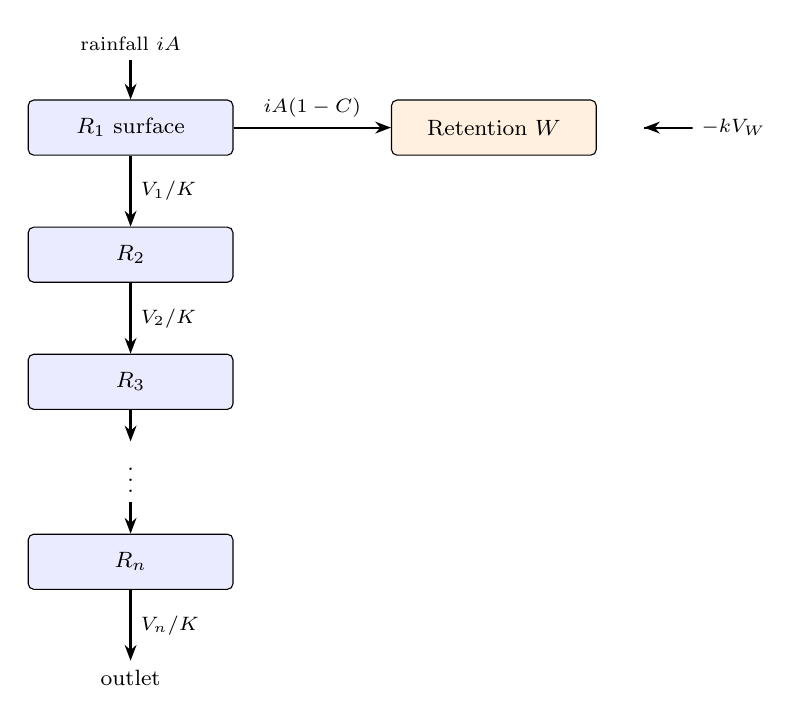
\begin{tikzpicture}[
  node distance=9mm,
  blk/.style={draw,rounded corners=2pt,minimum width=26mm,minimum height=7mm,font=\footnotesize},
  ret/.style={blk,fill=orange!12},
  res/.style={blk,fill=blue!8},
  ar/.style={-{Stealth[length=2mm]},thick}
]
\node[res] (r1) {$R_1$ surface};
\node[ret,right=20mm of r1] (w) {Retention $W$};
\node[res,below=of r1] (r2) {$R_2$};
\node[res,below=of r2] (r3) {$R_3$};
\node[below=4mm of r3,font=\footnotesize] (dots) {$\vdots$};
\node[res,below=4mm of dots] (rn) {$R_n$};
\node[below=of rn,font=\footnotesize] (out) {outlet};
\draw[ar] (r1) -- node[above,font=\scriptsize] {$iA(1-C)$} (w);
\draw[ar] ([xshift=6mm]w.east) .. controls +(8mm,0) and +(8mm,0) .. ([xshift=6mm]w.east)
   node[right=6mm,font=\scriptsize] {$-kV_W$};
\draw[ar] (r1) -- node[right,font=\scriptsize] {$V_1/K$} (r2);
\draw[ar] (r2) -- node[right,font=\scriptsize] {$V_2/K$} (r3);
\draw[ar] (r3) -- (dots);
\draw[ar] (dots) -- (rn);
\draw[ar] (rn) -- node[right,font=\scriptsize] {$V_n/K$} (out);
\node[above=5mm of r1,font=\scriptsize] (rain) {rainfall $iA$};
\draw[ar] (rain) -- (r1);
\end{tikzpicture}
\end{center}

\subsection{Types}

All are defined in \exfile{resources/cn\_catchment.json}.

\begin{longtable}{@{}p{0.27\textwidth}p{0.15\textwidth}p{0.50\textwidth}@{}}
\toprule
\textbf{Type} & \textbf{Kind} & \textbf{Role}\\
\midrule
\endhead
\code{CN\_retention} & block & Abstraction store $V_W$. Carries $CN$, computes
$S$, $I_a$, $W$ and the runoff fraction $C$, and applies the drying loss.\\
\code{CN\_reservoir} & block & One linear reservoir of the cascade; discharge
$V/K$. The first also receives the rainfall.\\
\code{CN\_partition\_link} & link & Carries $i\,A\,(1-C)$ from the surface
reservoir to the retention store. Flow expression
\code{Precipitation.s*(1-C.e)}.\\
\code{CN\_cascade\_link} & link & Discharge \code{Storage.s/K.s} between
successive reservoirs.\\
\code{CN\_outlet} & link & The outlet hydrograph, \code{Storage.s/K.s} from the
last reservoir. The only way water leaves the component.\\
\code{CN\_Catchment} & composite & $n=5$, matched to the NRCS peak.\\
\code{CN\_Catchment\_3} & composite & $n=3$, lighter, flatter peak.\\
\bottomrule
\end{longtable}

\noindent
The partition happens in a \emph{link} rather than a block because the runoff
fraction depends on the rainfall rate, held by the surface reservoir, and on
$W$, held by the retention store. A link expression can see both endpoints;
a block expression cannot reach another block.

\subsection{Ports}

External connections resolve by link type:

\begin{center}
\begin{tabular}{@{}lll@{}}
\toprule
\textbf{Link type} & \textbf{Direction} & \textbf{Attaches to}\\
\midrule
\code{CN\_outlet} & out of the composite & the last reservoir $R_n$\\
\code{CN\_outlet} & into the composite & the surface reservoir $R_1$\\
any other (\code{*}) & into the composite & the surface reservoir $R_1$\\
\bottomrule
\end{tabular}
\end{center}

\noindent
Because the fallback offers no outward direction, \code{CN\_outlet} is the only
way water leaves a catchment. It attaches inbound as well, so the outlet of one
catchment may discharge directly into the next one downstream. Inflow of any
kind enters the surface reservoir and is routed onward without being subjected
to the curve number partition, which applies to rainfall only --- water arriving
from upstream has already had its abstraction taken out.

\subsection{Parameters}

\begin{longtable}{@{}p{0.30\textwidth}p{0.20\textwidth}p{0.42\textwidth}@{}}
\toprule
\textbf{Property} & \textbf{Units} & \textbf{Notes}\\
\midrule
\endhead
\code{CN} & --- & Curve number, usable range about 30--98. Sets $S$ and
$I_a=0.2S$ and enters the lag equation. $S\to0$ at $CN=100$.\\
\code{area} & m$^2$, ft$^2$, km$^2$ & Applied to every member.\\
\code{hydraulic\_length} & m, ft, km, yd & Longest flow path $\ell$; with $CN$
and slope it sets $L$ and hence every $K=L/(n-1)$.\\
\code{slope} & --- & Dimensionless rise over run; converted to percent
internally for the lag equation.\\
\code{recovery\_coefficient} & 1/day, 1/hr & Drying rate $k$.\\
\code{initial\_abstraction\_depth} & m, mm, in, ft & Antecedent condition;
zero means the first $0.2S$ of rain yields no runoff.\\
\code{Precipitation} & --- & Precipitation source, applied to $R_1$.\\
\bottomrule
\end{longtable}

\noindent
All values are held internally in metres and days. Outflow is reported with the
usual flow units, \code{m\textasciicircum3/day;ft\textasciicircum3/s;m\textasciicircum3/s}.

\subsection{Outputs}

Useful reported quantities include, on the retention member, $S$, $I_a$, $W$,
$C$ and the drying loss; on each reservoir, the stored volume, equivalent depth
and discharge; and on the outlet link, the flow, which is the hydrograph.

\section{Verification}

A uniform design storm of $240$~mm over 24~hours on a $10$~ha catchment with
$CN=75$ and drying disabled, so that the analytical result is unambiguous. Here
$S=84.7$~mm, $I_a=16.9$~mm and $P_e=223.1$~mm, giving $Q=161.7$~mm from
\eqref{eq:scs}.

\begin{center}
\begin{tabular}{@{}lrrr@{}}
\toprule
& \textbf{simulated} & \textbf{analytical} & \textbf{difference}\\
\midrule
abstraction & 7826.4 m$^3$ & 7830.6 m$^3$ & 0.05\%\\
runoff & 16185.6 m$^3$ & 16169.4 m$^3$ & 0.10\%\\
total (mass balance) & 24012.0 m$^3$ & 24000.0 m$^3$ & 0.05\%\\
\bottomrule
\end{tabular}
\end{center}

\noindent
The residuals are at the level of the solver tolerance. The residence time was
also checked: for $\ell=1000$~m, $CN=75$ and $s=0.02$ the lag equation gives
$L=0.02812$~day ($0.675$~hr) and the model assigned $K=0.007030$~day $=L/4$.

\paragraph{Not yet verified.} The peak timing and shape of the hydrograph
follow by construction from $K=L/(n-1)$, but have not been confirmed
numerically. That check is best done by inspecting the outlet flow series in
the interface.

\section{Worked usage}

\begin{lstlisting}[style=plain]
create source;type=Precipitation,name=Rain,timeseries=precipitation.csv
create composite;type=CN_Catchment,name=Cat1,x=200,y=0,
    CN=75,area=100000[m~^2],hydraulic_length=1000[m],slope=0.02,
    recovery_coefficient=0.1[1/day],initial_abstraction_depth=0,Precipitation=Rain
create link;from=Cat1,to=Outlet,type=CN_outlet,name=Outflow
\end{lstlisting}

\noindent
Catchments may be chained: a \code{CN\_outlet} from one may discharge into
another, whose surface reservoir routes the incoming flow onward.

\medskip
\noindent
A complete model is in \exfile{Examples/CN\_Catchment/CN\_watershed.ohq}: a
rural catchment discharging into an urban one and on to the watershed outlet,
alongside a third catchment that repeats the rural parameters with the
three-reservoir variant so the two cascades can be compared on one plot. The
folder \exdir{Examples/CN\_Catchment} also holds the design storm used to drive
it.

\section{Assumptions and limitations}

\begin{itemize}[leftmargin=1.4em]
\item \textbf{Curve number closure.} $I_a=0.2S$ is assumed. Studies favouring
$\lambda=0.05$ would require a different closure and a re-fitted $S$.
\item \textbf{Recovery is empirical.} The exponential drying term has no basis
in the curve number method itself; it is the device that lets an event method
run continuously, and $k$ is a calibration parameter. Recovered water leaves
the model.
\item \textbf{Antecedent moisture} is represented only through the state of
the abstraction store. There is no AMC~I/II/III switching.
\item \textbf{Shape versus peak.} The cascade matches the NRCS peak ordinate
with $n=5$; it is not a term-by-term reproduction of the dimensionless
hydrograph ordinates.
\item \textbf{The lag equation} is calibrated for catchments below roughly
$800$~ha with $CN$ between 50 and 95.
\item \textbf{No baseflow, no channel routing, no snow.} The component
produces direct runoff from a single catchment only.
\item \textbf{Uniform rainfall} over the catchment is assumed, as in the
original method.
\end{itemize}

\end{document}
